\documentclass[english,notitlepage]{revtex4-1}  % defines the basic parameters of the document
%For preview: skriv i terminal: latexmk -pdf -pvc filnavn



% if you want a single-column, remove reprint

% allows special characters (including æøå)
\usepackage[utf8]{inputenc}
%\usepackage[english]{babel}

%% note that you may need to download some of these packages manually, it depends on your setup.
%% I recommend downloading TeXMaker, because it includes a large library of the most common packages.

\usepackage{physics,amssymb}  % mathematical symbols (physics imports amsmath)
\include{amsmath}
\usepackage{graphicx}         % include graphics such as plots
\usepackage{xcolor}           % set colors
\usepackage{hyperref}         % automagic cross-referencing (this is GODLIKE)
\usepackage{listings}         % display code
\usepackage{subcaption}        % better subfigure support
\usepackage{float}
%\usepackage[section]{placeins}
\usepackage{algorithm}
\usepackage[noend]{algpseudocode}
\usepackage{subcaption}
\usepackage{tikz}
\usetikzlibrary{quantikz}
% defines the color of hyperref objects
% Blending two colors:  blue!80!black  =  80% blue and 20% black
\hypersetup{ % this is just my personal choice, feel free to change things
    colorlinks,
    linkcolor={red!50!black},
    citecolor={blue!50!black},
    urlcolor={blue!80!black}}

%% Defines the style of the programming listing
%% This is actually my personal template, go ahead and change stuff if you want



%% USEFUL LINKS:
%%
%%   UiO LaTeX guides:        https://www.mn.uio.no/ifi/tjenester/it/hjelp/latex/
%%   mathematics:             https://en.wikibooks.org/wiki/LaTeX/Mathematics

%%   PHYSICS !                https://mirror.hmc.edu/ctan/macros/latex/contrib/physics/physics.pdf

%%   the basics of Tikz:       https://en.wikibooks.org/wiki/LaTeX/PGF/Tikz
%%   all the colors!:          https://en.wikibooks.org/wiki/LaTeX/Colors
%%   how to draw tables:       https://en.wikibooks.org/wiki/LaTeX/Tables
%%   code listing styles:      https://en.wikibooks.org/wiki/LaTeX/Source_Code_Listings
%%   \includegraphics          https://en.wikibooks.org/wiki/LaTeX/Importing_Graphics
%%   learn more about figures  https://en.wikibooks.org/wiki/LaTeX/Floats,_Figures_and_Captions
%%   automagic bibliography:   https://en.wikibooks.org/wiki/LaTeX/Bibliography_Management  (this one is kinda difficult the first time)
%%   REVTeX Guide:             http://www.physics.csbsju.edu/370/papers/Journal_Style_Manuals/auguide4-1.pdf
%%
%%   (this document is of class "revtex4-1", the REVTeX Guide explains how the class works)


%% CREATING THE .pdf FILE USING LINUX IN THE TERMINAL
%%
%% [terminal]$ pdflatex template.tex
%%
%% Run the command twice, always.
%% If you want to use \footnote, you need to run these commands (IN THIS SPECIFIC ORDER)
%%
%% [terminal]$ pdflatex template.tex
%% [terminal]$ bibtex template
%% [terminal]$ pdflatex template.tex
%% [terminal]$ pdflatex template.tex
%%
%% Don't ask me why, I don't know.

\begin{document}

\title{FYS3150/4150 Project 2}      % self-explanatory
\author{Johannes Schäfers, Ferdinand Nilius, Michał Kiedrzyński}          % self-explanatory
\date{\today}                             % self-explanatory
\noaffiliation                            % ignore this, but keep it.


\maketitle 
    
\textit{All code for Project 2 can be found under: \url{https://github.uio.no/johascha/CompPhys/tree/master/Project_2}}.
    
\section*{Problem 1}

In order to rewrite the equation: 

\begin{equation} \label{eq: unscaled}
    	\gamma \frac{d^2u}{dx^2} = - F u(x)
\end{equation}
into a scaled form, where 
\begin{equation*}
    	\hat{x} = \frac{x}{L},    
\end{equation*}
the second derivative of $u(x)$ with respect to the new variable $\hat{x}$ must be found. This can be done as follows:
\begin{equation*}
    \frac{d^2u(x)}{d^2x}  =  \frac{d^2u(\hat{x})}{d^2\hat{x}} \cdot \frac{d\hat{x}}{dx} \cdot \frac{d\hat{x}}{dx} = \frac{d^2u(\hat{x})}{d^2\hat{x}} \cdot L^{-2}.
\end{equation*}
Substituting this into equation (\ref{eq: unscaled}) and reforming the equation yields:
\begin{equation*}
    \frac{d^2u(\hat{x})}{d^2\hat{x}}  =  - \frac{F \cdot L^2}{\gamma} u(\hat{x}) = - \lambda u(\hat{x}).
\end{equation*}
Here, $\lambda$ is used as a new constant that incorporates the term $\frac{F \cdot L^2}{\gamma}$.

\section*{Problem 2}
The code consists of two main parts. Implementing the 6 x 6 matrix and solving the eigenvalues as well as the eigenvectors. 
Therefore, we decided to use the armadillo library, which calculates the eigenvectors and eigenvalues of A.
A is given as the following matrix:
\begin{equation}
\label{eq:task2}
A = \frac{1}{h^2} 
\begin{bmatrix} 
 2 & -1 &  0 &  0 &  0 &  0 \\
-1 &  2 & -1 &  0 &  0 &  0 \\
 0 & -1 &  2 & -1 &  0 &  0 \\
 0 &  0 & -1 &  2 & -1 &  0 \\
 0 &  0 &  0 & -1 &  2 & -1 \\
 0 &  0 &  0 &  0 & -1 &  2
\end{bmatrix}.  
\end{equation}

Running the algorithm shows that the analytical solution is identical to 
the numeric solution (up to 6 decimal places, see Table \ref{tab:task2}), which was calculated using the Armadillo library. Differences between the two solutions only show, after 14 decimal places. These are likely caused by rounding errors.

\begin{table}[H]
\centering
\begin{tabular}{cccc}
\hline
$j$ & Analytical $\lambda_j$ & Numerical $\lambda_j$ & Absolute Difference \\
\hline
1 & $9.705050\times 10^{0}$  & $9.705050\times 10^{0}$  & $3.55 \times 10^{-15}$ \\
2 & $3.689799\times 10^{1}$ & $3.689799\times 10^{1}$ & $2.13 \times 10^{-14}$ \\
3 & $7.619294\times 10^{1}$ & $7.619294\times 10^{1}$ & $1.42 \times 10^{-14}$ \\
4 & $1.198070\times 10^{2}$ & $1.198070\times 10^{2}$ & $2.84 \times 10^{-15}$ \\
5 & $1.591020\times 10^{2}$ & $1.591020\times 10^{2}$ & $0.00 \times 10^{0}$ \\
6 & $1.862949\times 10^{2}$ & $1.862949\times 10^{2}$ & $5.68 \times 10^{-14}$ \\
\hline
\end{tabular}
\caption{Comparison of analytical and numerical eigenvalues for $N = 6$.}
\label{tab:task2}
\end{table}


\section*{Problem 3} 
\subsection*{Task a)}
Since the matrix remains the same throughout the algorithm, it can be used as a constant. The algorithm uses two loops, one for the rows and one for the columns, 
to create a grid search, using the matrix element $k = 0, l = 1$ as an initial value, while checking all other elements from the bottom upward afterwards. If the algorithm finds a larger absolute value, the variable containing the maximum value of $\bold{A}$, as well as the two variables that hold the indices of the said element, are updated. After all elements above the diagonal have been checked, the algorithm returns the largest absolute value.

\subsection*{Task b)}
The given matrix $\bold{A}$ is:

$$
\bold{A} = 
\begin{bmatrix}
1 & 0 & 0 & 0.5 \\
0 & 1 & -0.7 & 0 \\
0 & -0.7 & 1 & 0 \\
0.5 & 0 & 0 & 1
\end{bmatrix}
$$

Obviously, the absolute highest value without the main diagonal is $-0.7$, the algorithm in the previous section delivers successfully the same value.

\section*{Problem 4}
\subsection*{Task a)}
The implementation of the Jacobi Rotation Algorithm can be described as follows:
Starting with the variable $\tau$, which is given as:
$$
\tau = \frac{A_{ll} - A_{kk}}{2A_{kl}}
$$
Where $A_{kl}$ is the largest non diagonal element of the matrix $A$.
Now the goal is to select the smaller root of the quadratic equation for the tangent parameter t in the Jacobi Rotation Algorithm. It uses different formulations for positive and negative tau to prevent numerical loss of significance.
$$
t = \tan(\tau) = \begin{cases} 
\frac{1}{\tau + \sqrt{1 + \tau^2}} & \text{if } \tau \geq 0 \\ 
\frac{-1}{-\tau + \sqrt{1 + \tau^2}} & \text{if } \tau < 0 
\end{cases}
$$
Out of this quadratic equation the solution for the parameter c and s are the following. Hereby $c= \cos{(\theta)}$ and $s= \sin{(\theta)}$ are the roation parameters.
$$
c = \frac{1}{\sqrt{1 + t^2}} \newline
$$
$$
s = c \cdot t
$$
In the following steps, the matrix elements are updated by the algorithm. 
Especially the two diagonal elements at indices $(k,k)$ and $(l,l)$ are altered by the rotation.
$$
A_{kk}' = A_{kk}c^2 - 2A_{kl}cs + A_{ll}s^2
$$

$$
A_{ll}' = A_{ll}c^2 + 2A_{kl}cs + A_{kk}s^2
$$
The largest off-diagonal elements are forced to zero, which is the main objective of the rotation step.
$$
A_{kl}' = A_{lk}' = 0.0
$$
Updating all other elements in row $l$ and column $l$ to account for how the rotation mixes the indices $k$ and $l$ 
$$
A_{ik}' = A_{ki}' = A_{ik}c - A_{il}s \quad \text{for } i \neq k,l
$$
Same for $l$
$$
A_{il}' = A_{li}' = A_{il}c + A_{ik}s \quad \text{for } i \neq k,l
$$
Finally, the eigenvector matrix $\bold{R}$ is updated. Each column of $\bold{R}$ represents an eigenvector corresponding to an eigenvalue in $\bold{A}$. You have to apply the same rotations to $\bold{R}$ as you did to $\bold{A}$.
\begin{align*}
R_{ik}' &= R_{ik}c - R_{il}s \quad \text{for all } i \\
R_{il}' &= R_{il}c + R_{ik}s \quad \text{for all } i
\end{align*}

A short summary of the Jacobi Rotation Algorithm as pseudo-code can be described as the following:
\begin{figure}[H]
    \begin{algorithm}[H]
        \caption{Jacobi Rotation Algorithm}
        \label{algo:Jacobi}

        \begin{algorithmic}[1]
            \Require Symmetric matrix $A \in \mathbb{R}^{n \times n}$,
                     tolerance $\varepsilon$
            \Ensure Diagonal matrix $D$ and eigenvector matrix $R$

            \State $R \gets I_n$

            \While{$\max_{i \neq j}|A_{ij}| > \varepsilon$}

                \State $(k,l) \gets
                    \underset{1 \leq i < j \leq n}{\arg\max}\,
                    |A_{ij}|$

                \State $\tau \gets
                    \dfrac{A_{ll}-A_{kk}}{2A_{kl}}$

                \If{$\tau \geq 0$}
                    \Statex \hspace{\algorithmicindent}\hspace{\algorithmicindent} $t \gets
                        \dfrac{1}{\tau+\sqrt{1+\tau^2}}$
                \Else
                    \Statex \hspace{\algorithmicindent} \hspace{\algorithmicindent} $t \gets
                        -\dfrac{1}{-\tau+\sqrt{1+\tau^2}}$
                \EndIf

                \State $c \gets \dfrac{1}{\sqrt{1+t^2}}$
                \State $s \gets tc$

                \State $a \gets A_{kk}$, \quad
                       $d \gets A_{ll}$, \quad
                       $b \gets A_{kl}$

                \State $A_{kk} \gets a-2tb+t^2d$
                \State $A_{ll} \gets d+2tb+t^2a$
                \State $A_{kl} \gets 0$
                \State $A_{lk} \gets 0$

                \For{$i = 1, 2, \ldots, n, \, i \neq k,l$}
                    \State $a_i \gets A_{ki}$, \quad
                           $d_i \gets A_{li}$
                    \State $A_{ki} \gets a_i-td_i$
                    \State $A_{ik} \gets A_{ki}$
                    \State $A_{li} \gets d_i+ta_i$
                    \State $A_{il} \gets A_{li}$
                \EndFor

                \For{$i = 1, 2, \ldots, n$}
                    \State $r_i \gets R_{ki}$, \quad
                           $q_i \gets R_{li}$
                    \State $R_{ki} \gets r_i-tq_i$
                    \State $R_{li} \gets q_i+tr_i$
                \EndFor

            \EndWhile

            \State $D \gets A$
            \State \Return $D,R$
        \end{algorithmic}
    \end{algorithm}
\end{figure}






\subsection*{Task b)}
Using the same matrix as in Equation \ref{eq:task2}, the written algorithm generates the expected eigenvalues and eigenvectors. The outputs are saved to a .txt file, where they can be compared. The calculated eigenvalues can be seen in the table below:

\begin{table}[H]
\centering
\begin{tabular}{cccc}
\hline
$j$ & Analytical $\lambda_j$ & Numerical $\lambda_j$ & Absolute Difference \\
\hline
1 & $9.705050\times10^{0}$ & $9.705050\times10^{0}$ & $2.66\times10^{-14}$ \\
2 & $3.689799\times10^{1}$ & $3.689799\times10^{1}$ & $6.39\times10^{-14}$ \\
3 & $7.619294\times10^{1}$ & $7.619294\times10^{1}$ & $1.42\times10^{-14}$ \\
4 & $1.198070\times10^{2}$ & $1.198070\times10^{2}$ & $2.84\times10^{-14}$ \\
5 & $1.591020\times10^{2}$ & $1.591020\times10^{2}$ & $1.42\times10^{-13}$ \\
6 & $1.862949\times10^{2}$ & $1.862949\times10^{2}$ & $1.42\times10^{-13}$ \\
\hline
\end{tabular}
\caption{Comparison of analytical and numerical eigenvalues for $N = 6$.}\label{tab:task5}
\end{table}
From the absolute differences between the newly calculated numerical eigenvalues and the analytical eigenvalues listed in table \ref{tab:task5}, it can be seen that the new algorithm performs slightly worse than the implementation in the Armadillo library.  Similarly, the eigenvectors, which are also output into a .txt file, show only minor differences, with the largest individual per element difference being of magnitude $10^{-16}$, when the eigenvectors are normed to length $1$ in their L2-norm. Important to note is that the eigenvectors can be flipped, since the code does not check the orientation of the eigenvectors.

\section*{Problem 5}

\subsection*{a)}
\begin{figure}[H]
    \centering
    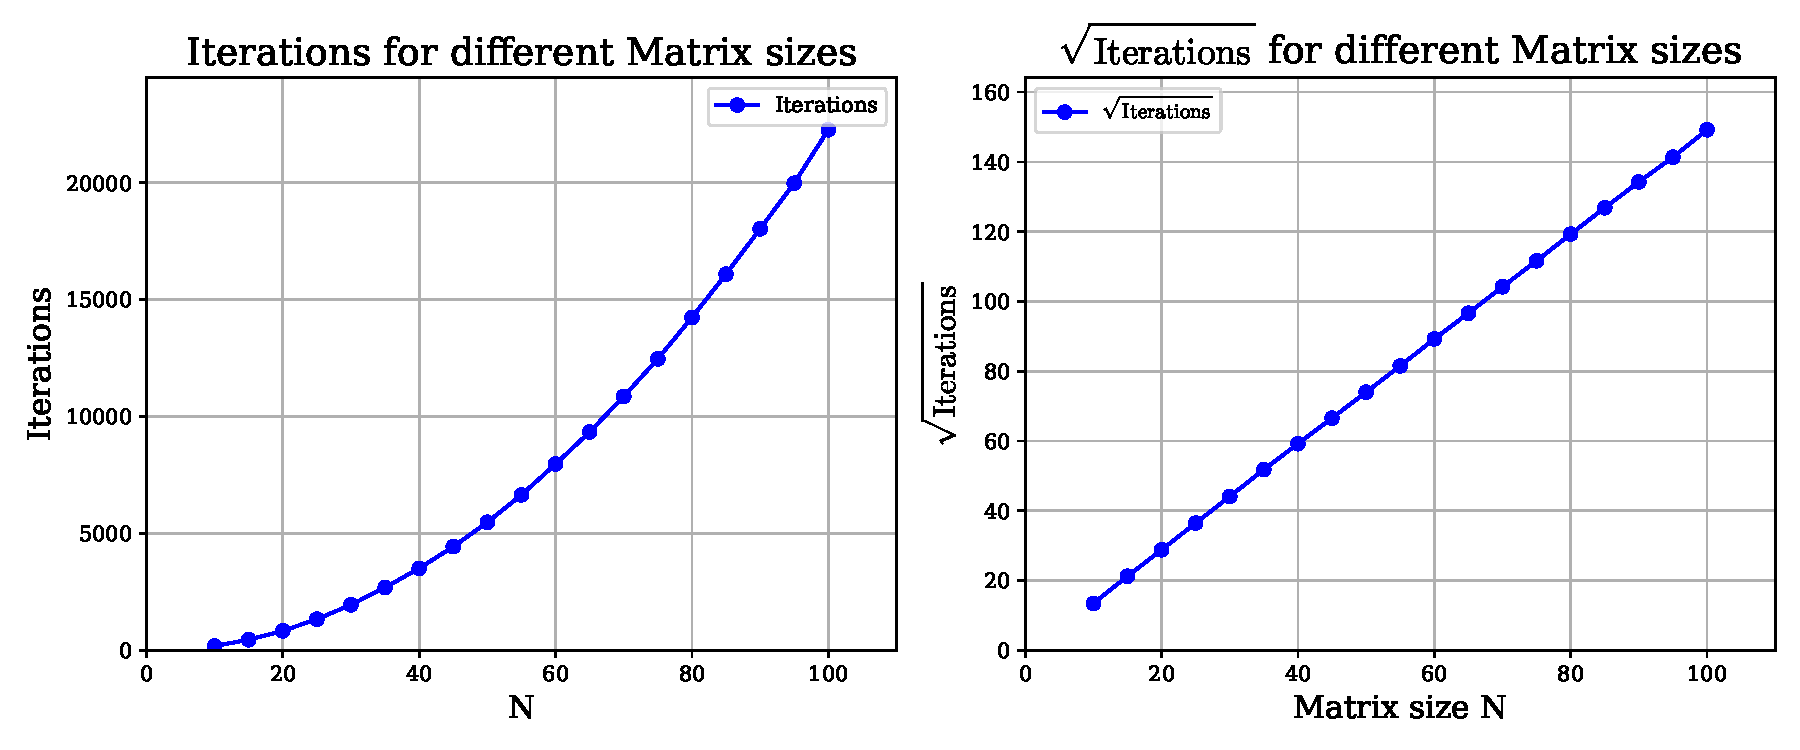
\includegraphics[width=0.7\linewidth]{task5a.pdf}
    \caption{Comparison between the matrix size and the number of iterations needed to find the eigenvectors for the tridiagonal matrix (left). Comparison between the matrix size and the square root of the number of iterations needed to find the eigenvectors for the tridiagonal matrix (right). }
    \label{fig:Iterationstridiag}
\end{figure}
In the plot above (Figure \ref{fig:Iterationstridiag}, left), it can be seen how the number of similarity transformations needed for the Jacobi Rotation Algorithm develops based on the size of the matrix. For this exercise the matrix, which has been presented in equation \ref{eq:task2}, was used and iterations were done until the largest off-diagonal element was smaller than $10^{-20}$. Taking the square root of the number of iterations and creating a similar plot (Figure \ref{fig:Iterationstridiag}, right) reveals a linear relationship. Therefore the assumption can be made that the number of iterations rises quadratically with the dimensions of the quadratic matrix. This is contradicted by \cite{golub2013matrix}, who argue that it takes $log(n)$ sweeps, where a sweep consists of $\frac{n(n-1)}{2}$ rotations. However, this scaling behavior, which would in total be equal to $\mathcal{O}(log(n)n^2)$ is not properly seen here as the plots only display the number of iterations for matrix sizes of up to $100\times 100$, where the logarithmic factor barely has an influence on the overall result.


\subsection*{b)}
\begin{figure}[H]
    \centering
    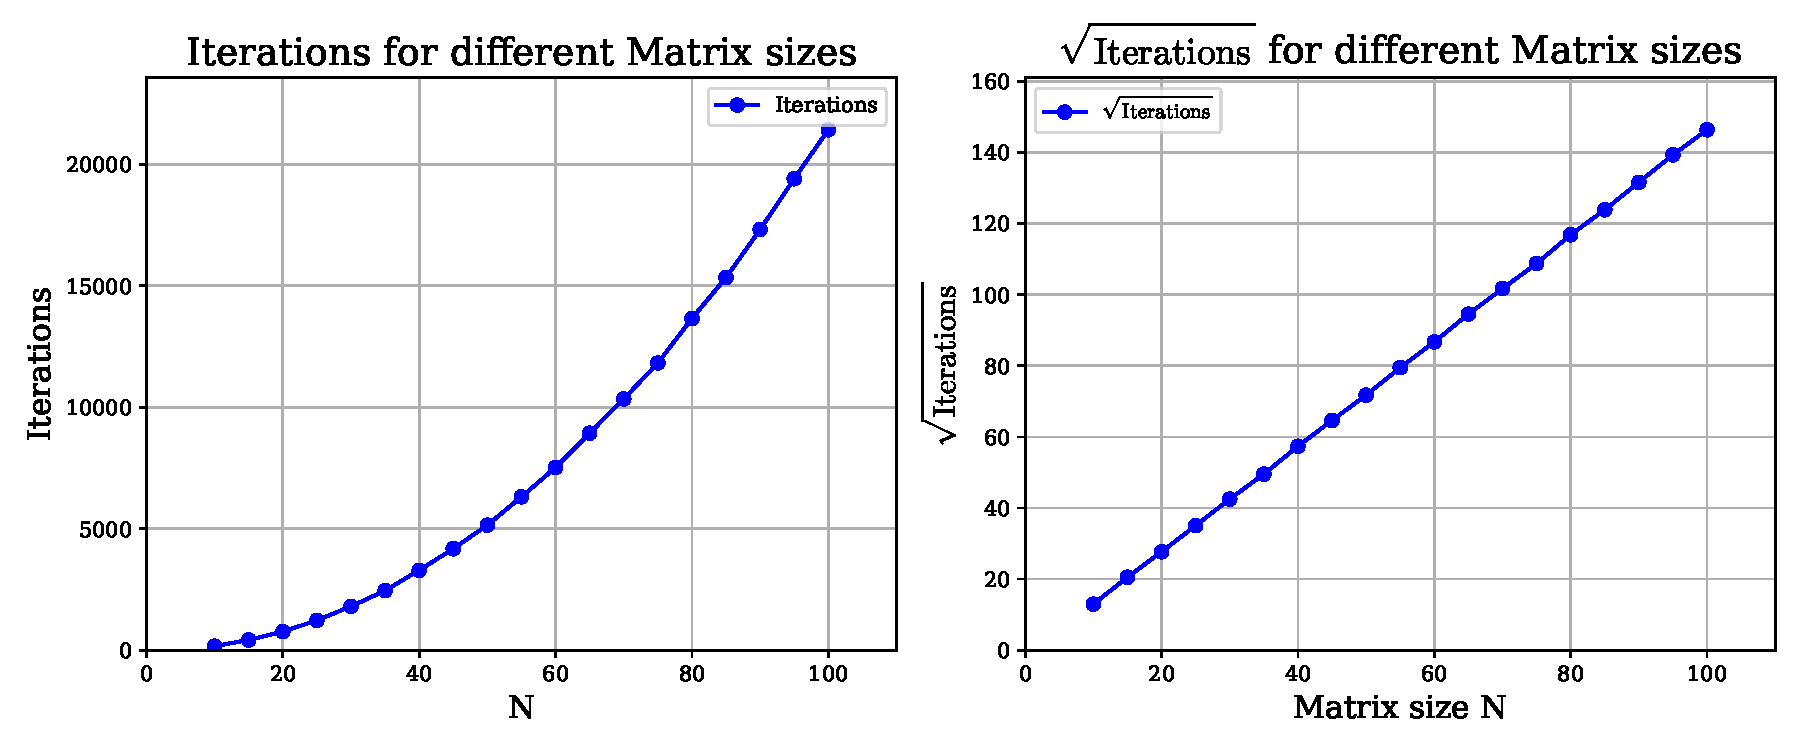
\includegraphics[width=0.7\linewidth]{task5b.pdf}
    \caption{Comparison between the matrix size and the number of iterations needed to find the eigenvectors for the random dense matrix (left). Comparison between the matrix size and the square root of the number of iterations needed to find the eigenvectors for the random dense matrix (right). }
    \label{fig:Iterationsrandom}
\end{figure}

When repeating the same process with a dense, random, and symmetric matrix, the scaling of the number of iterations with increasing matrix size remains the same. This phenomenon can be explained by the destruction of the tridiagonal structure under the rotations applied during the algorithm. As the algorithm does its first iteration on a tridiagonal, it will not only update the elements on the sub- and super-diagonal, but of elements on the same column or row as the largest element. Therefore after even a single step the tridiagonal structure is lost and the scaling is similar to a dense matrix.

\section*{Problem 6}

Using the following discretization:
$$
\frac{-v_{i+1}+2v_i-v_{v-1}}{h^2} = \lambda v_i
$$

we define the matrix $\mathbf{A_N} : (n-1\times n-1)$ as:

$$
\mathbf{A_N} = \frac{1}{h^2} 
\begin{bmatrix} 
 2 & -1 &  0 & \cdots & 0 \\
-1 &  2 & -1 & \ddots & \vdots \\
 0 & -1 & \ddots & \ddots & 0 \\
\vdots & \ddots & \ddots & 2 & -1 \\
 0 & \cdots & 0 & -1 & 2
\end{bmatrix}.
$$

Then, we apply the Jacobi solver from the previous tasks to compute the matrix's eigenvectors and eigenvalues. Figures \ref{fig:6_10} and \ref{fig:6_100} present the comparison of the calculated numerical result to the analytical solution. They present the eigenvectors associated with the three lowest eigenvalues, for $n=10$ and $n=100$ respectively. The resulting functions resemble the first three harmonics. 

\begin{figure}[htbp]
    \centering
    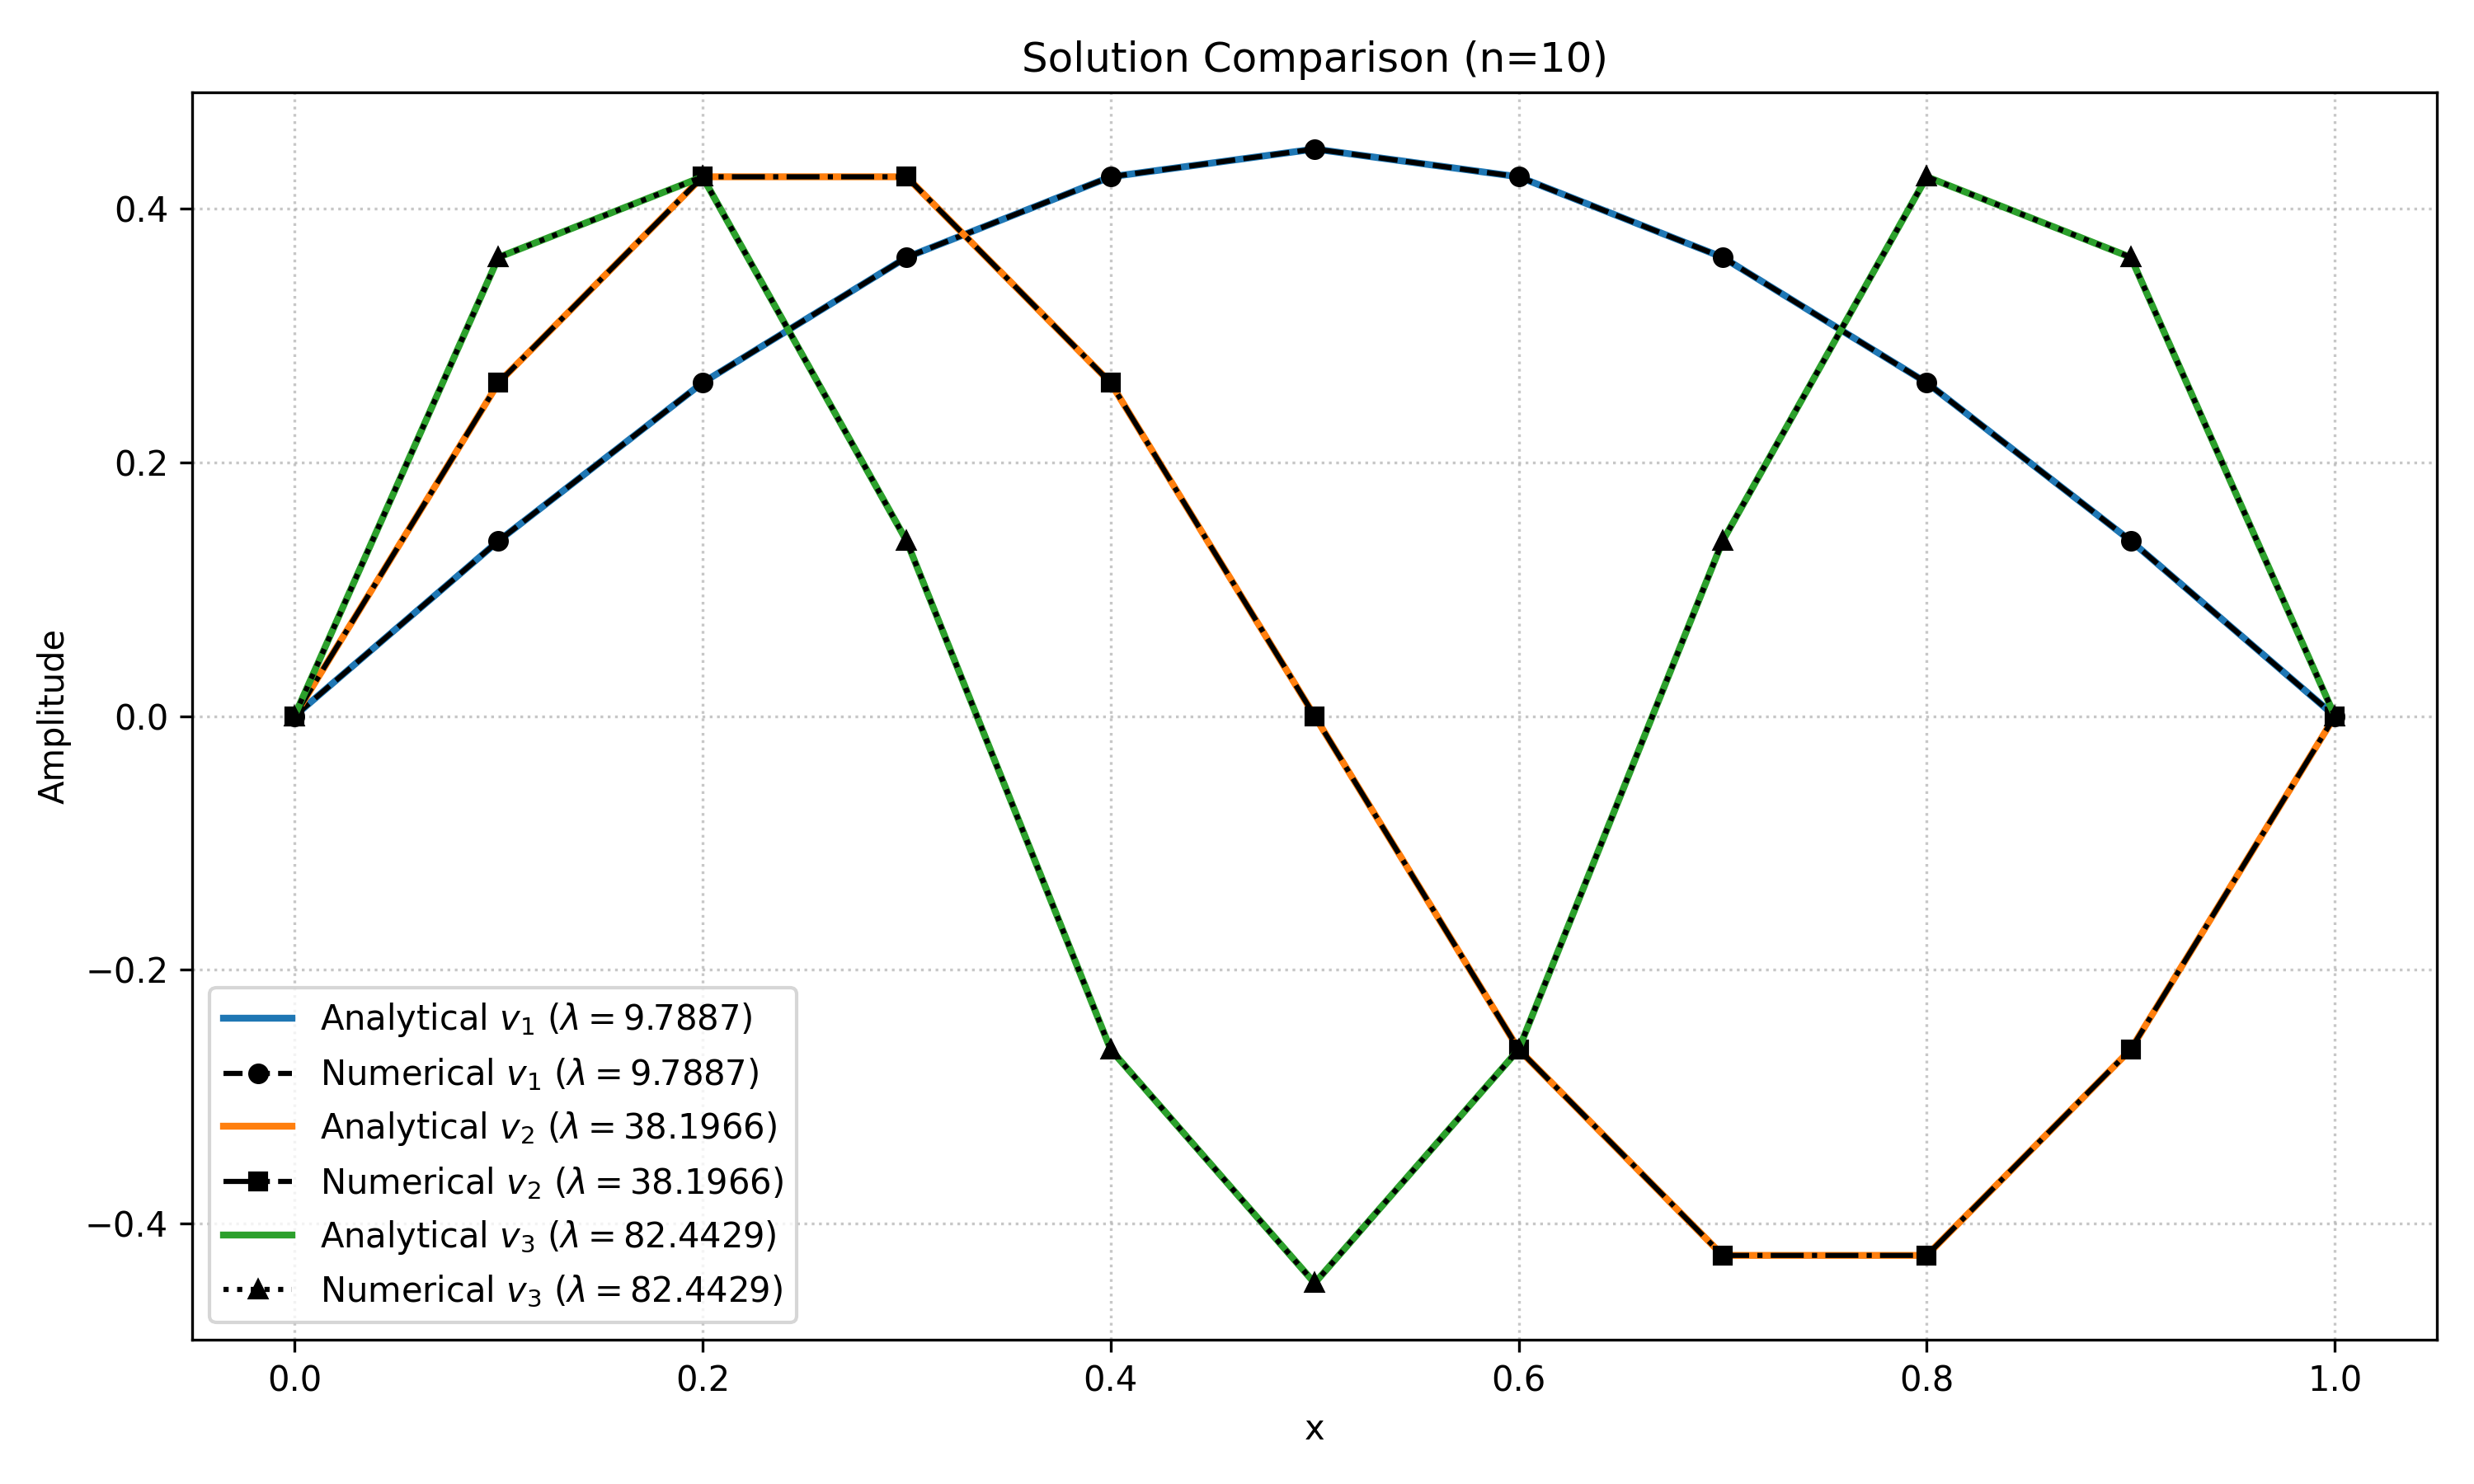
\includegraphics[width=1\textwidth]{task6_10.png}
    \caption{Comparison of analytical and numerical solutions for eigenvectors with three lowest eigenvalues (n=10) }
    \label{fig:6_10}
\end{figure}

\begin{figure}[htbp]
    \centering
    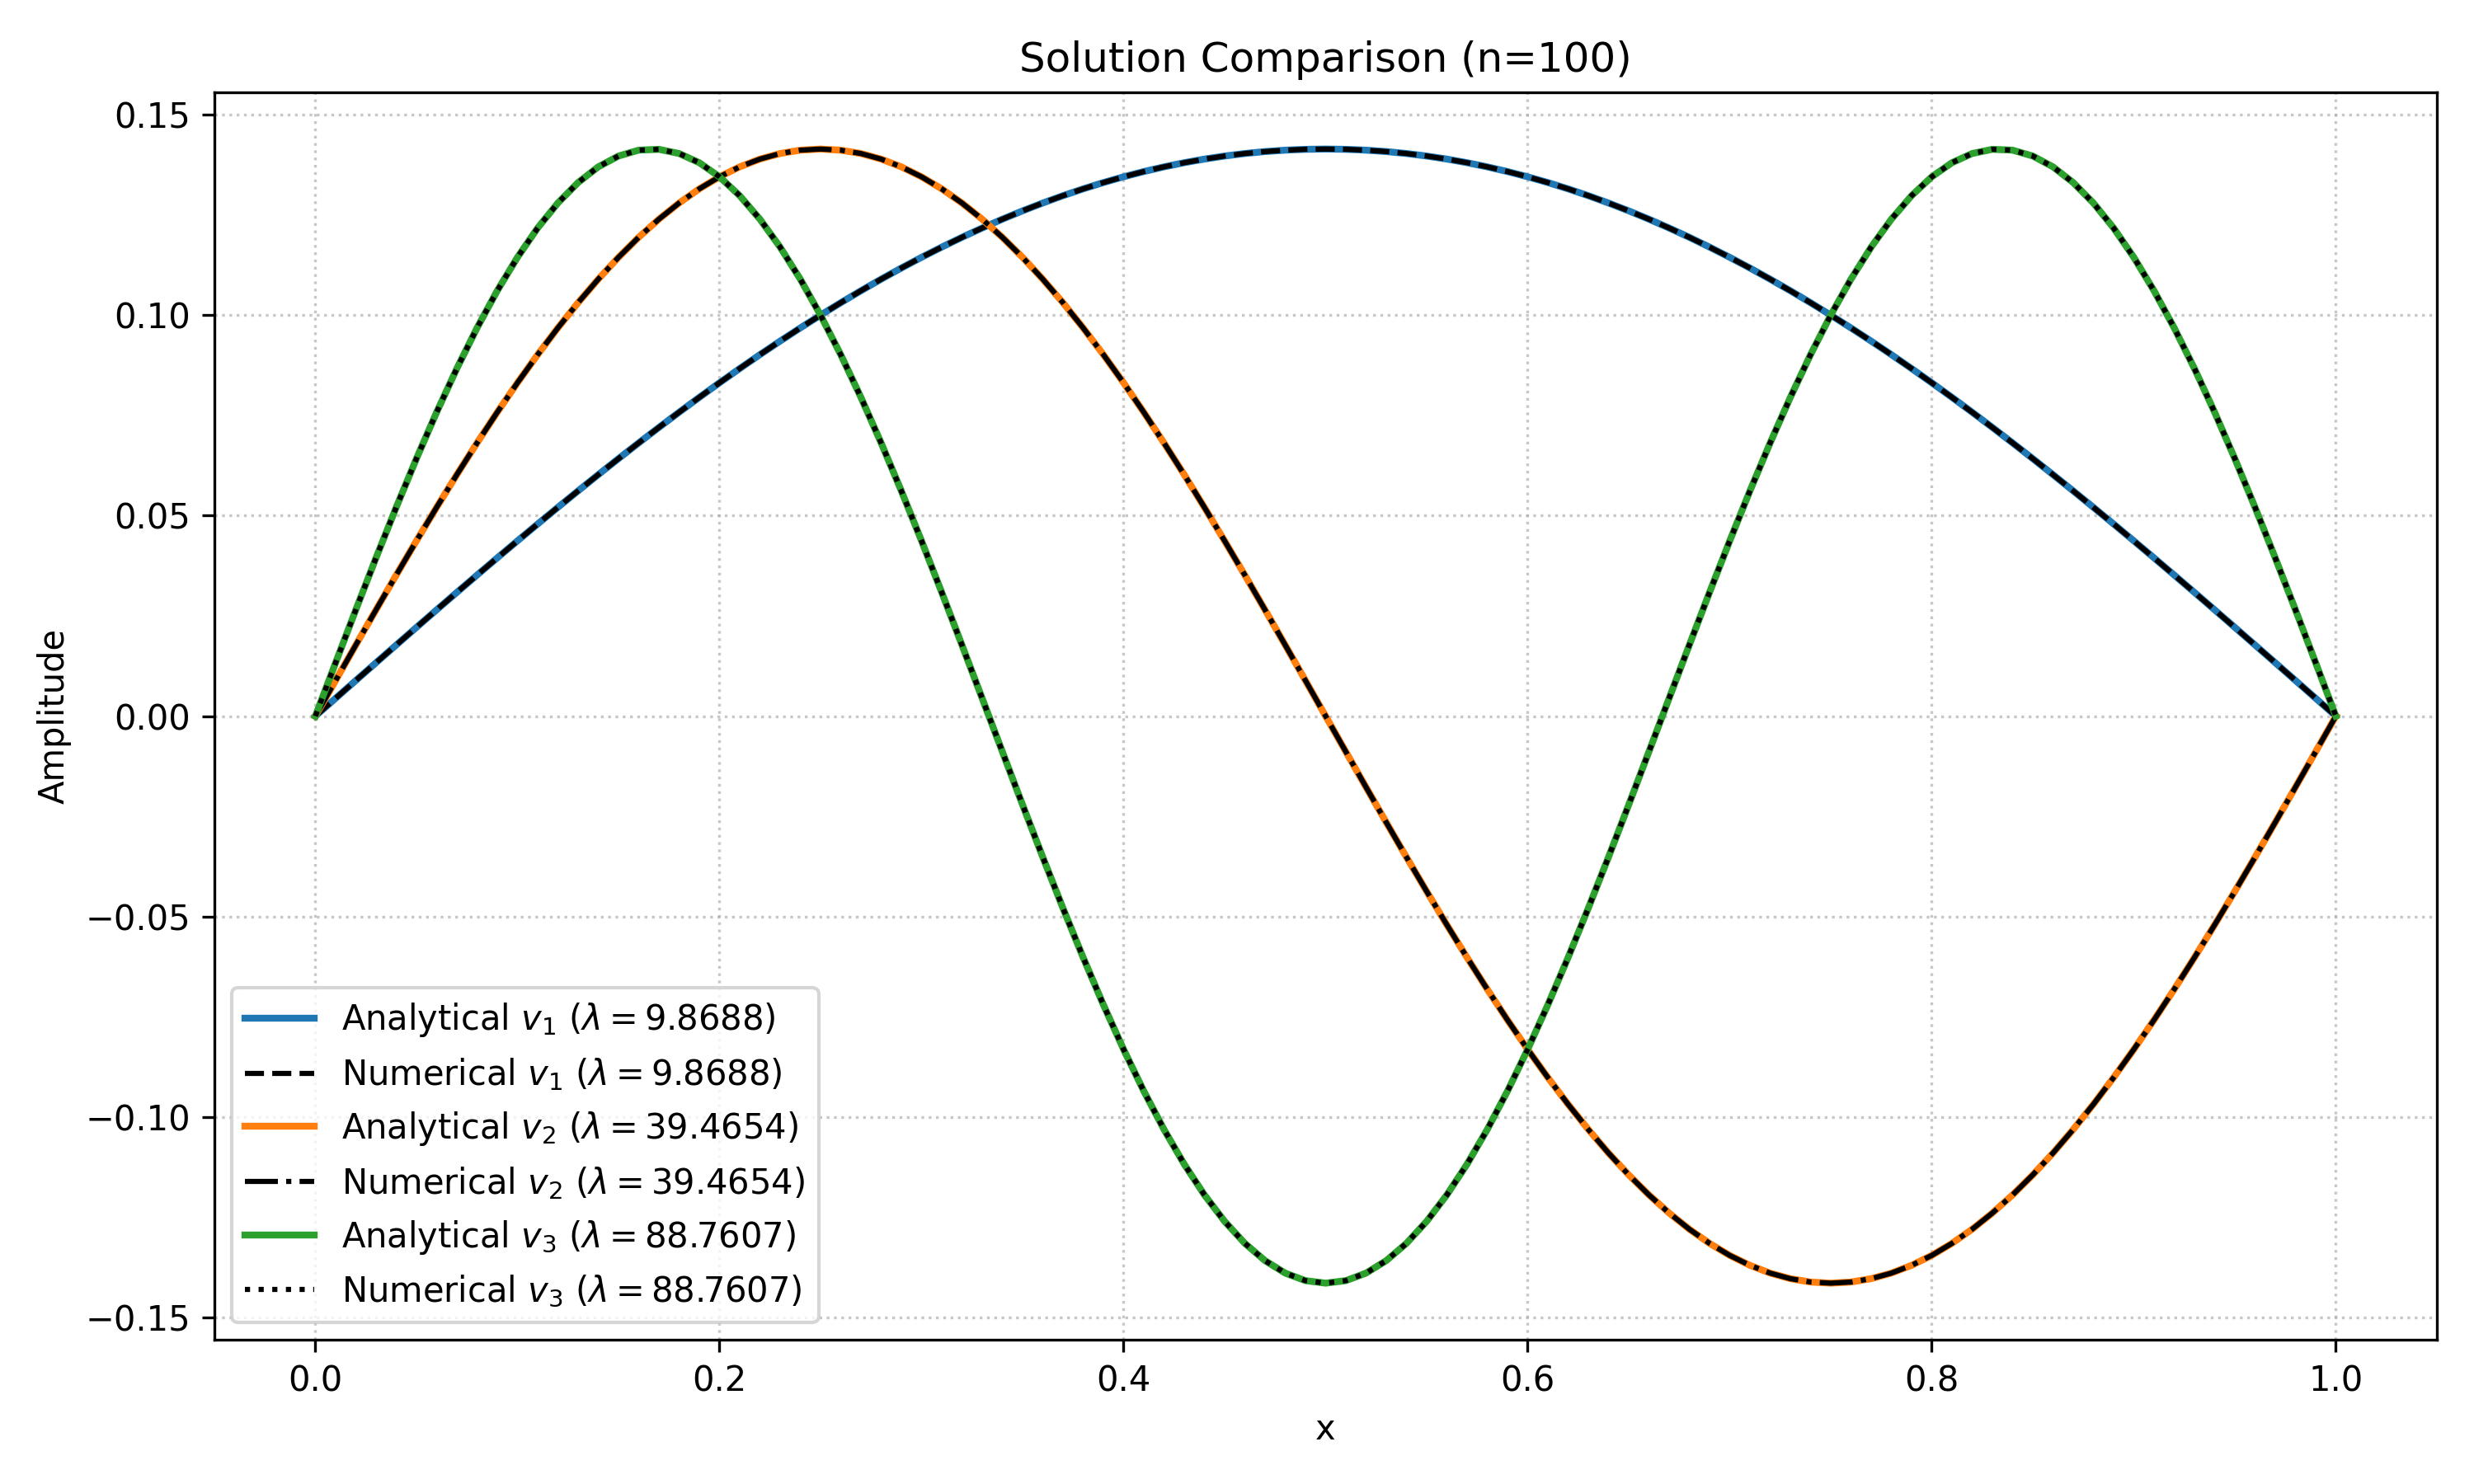
\includegraphics[width=1\textwidth]{task6_100.png}
    \caption{Comparison of analytical and numerical solutions for eigenvectors with three lowest eigenvalues (n=100) }
    \label{fig:6_100}
\end{figure}

% \begin{figure}[htbp]
%     \centering
%     \begin{subfigure}[b]{0.9\textwidth}
%         \centering
%         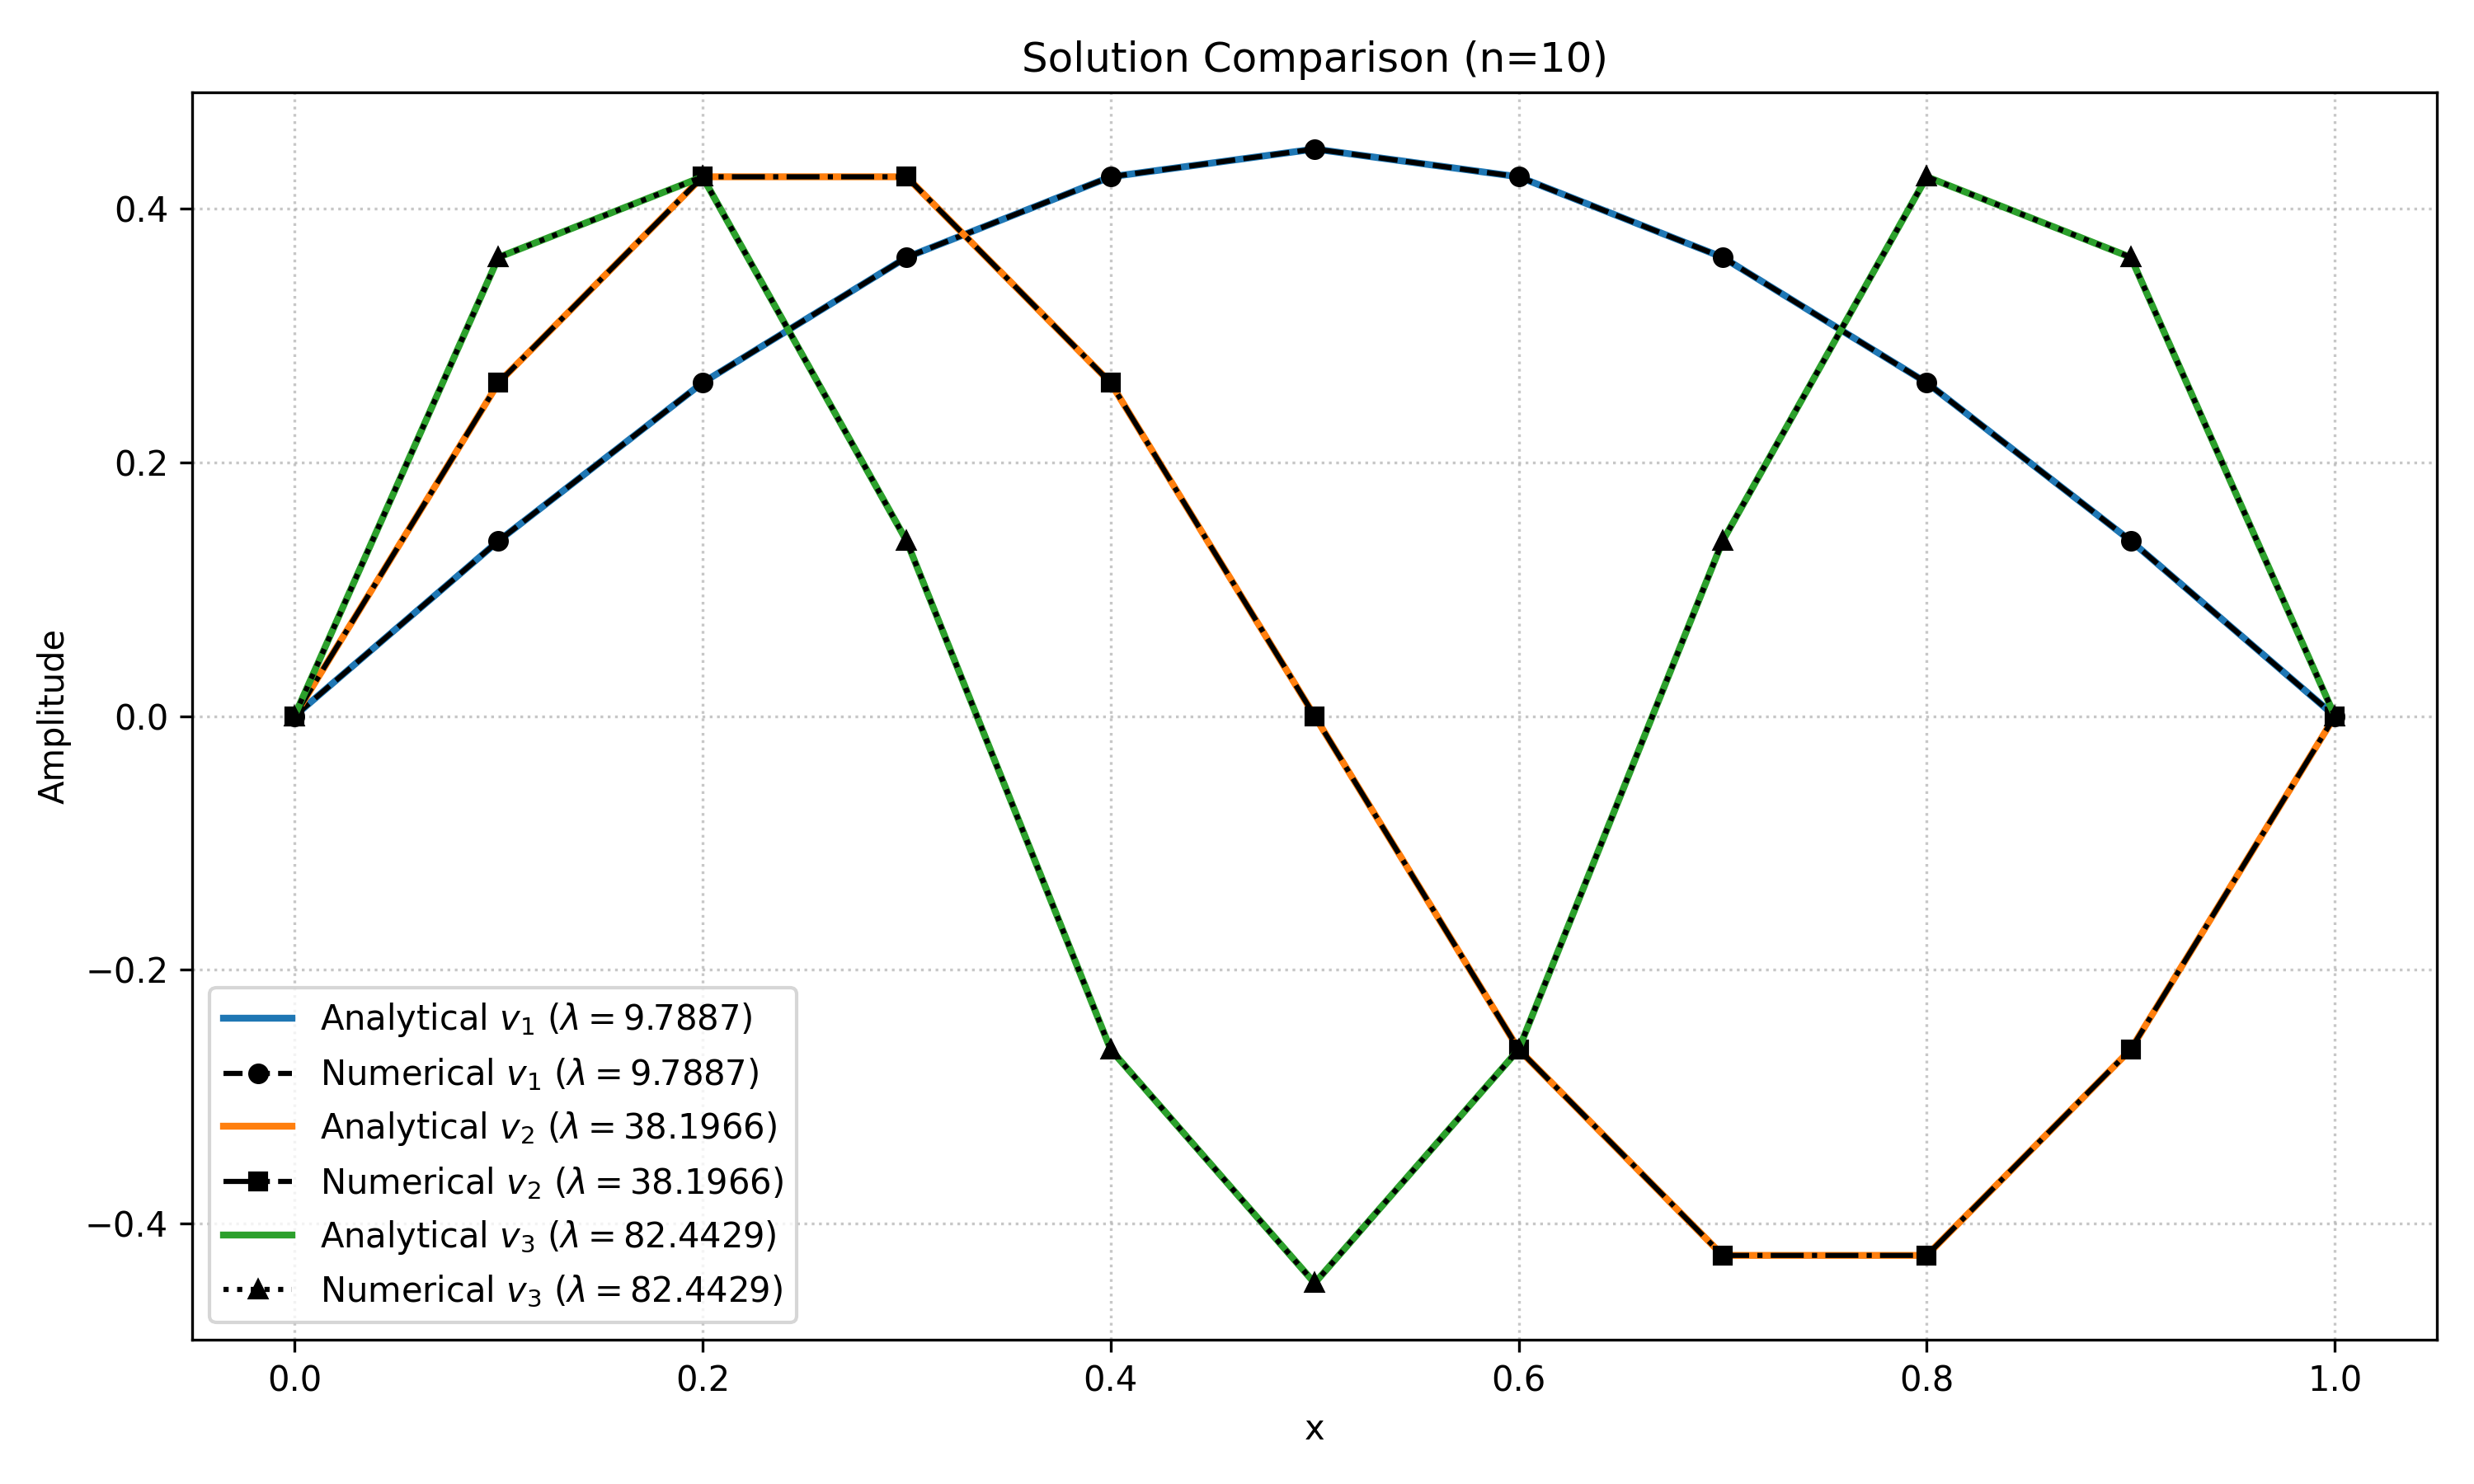
\includegraphics[width=1\textwidth]{task6_10.png}
%         \caption{Absolute error comparison, problem 8a}
%     \end{subfigure}
%     \begin{subfigure}[b]{0.9\textwidth}
%         \centering
%         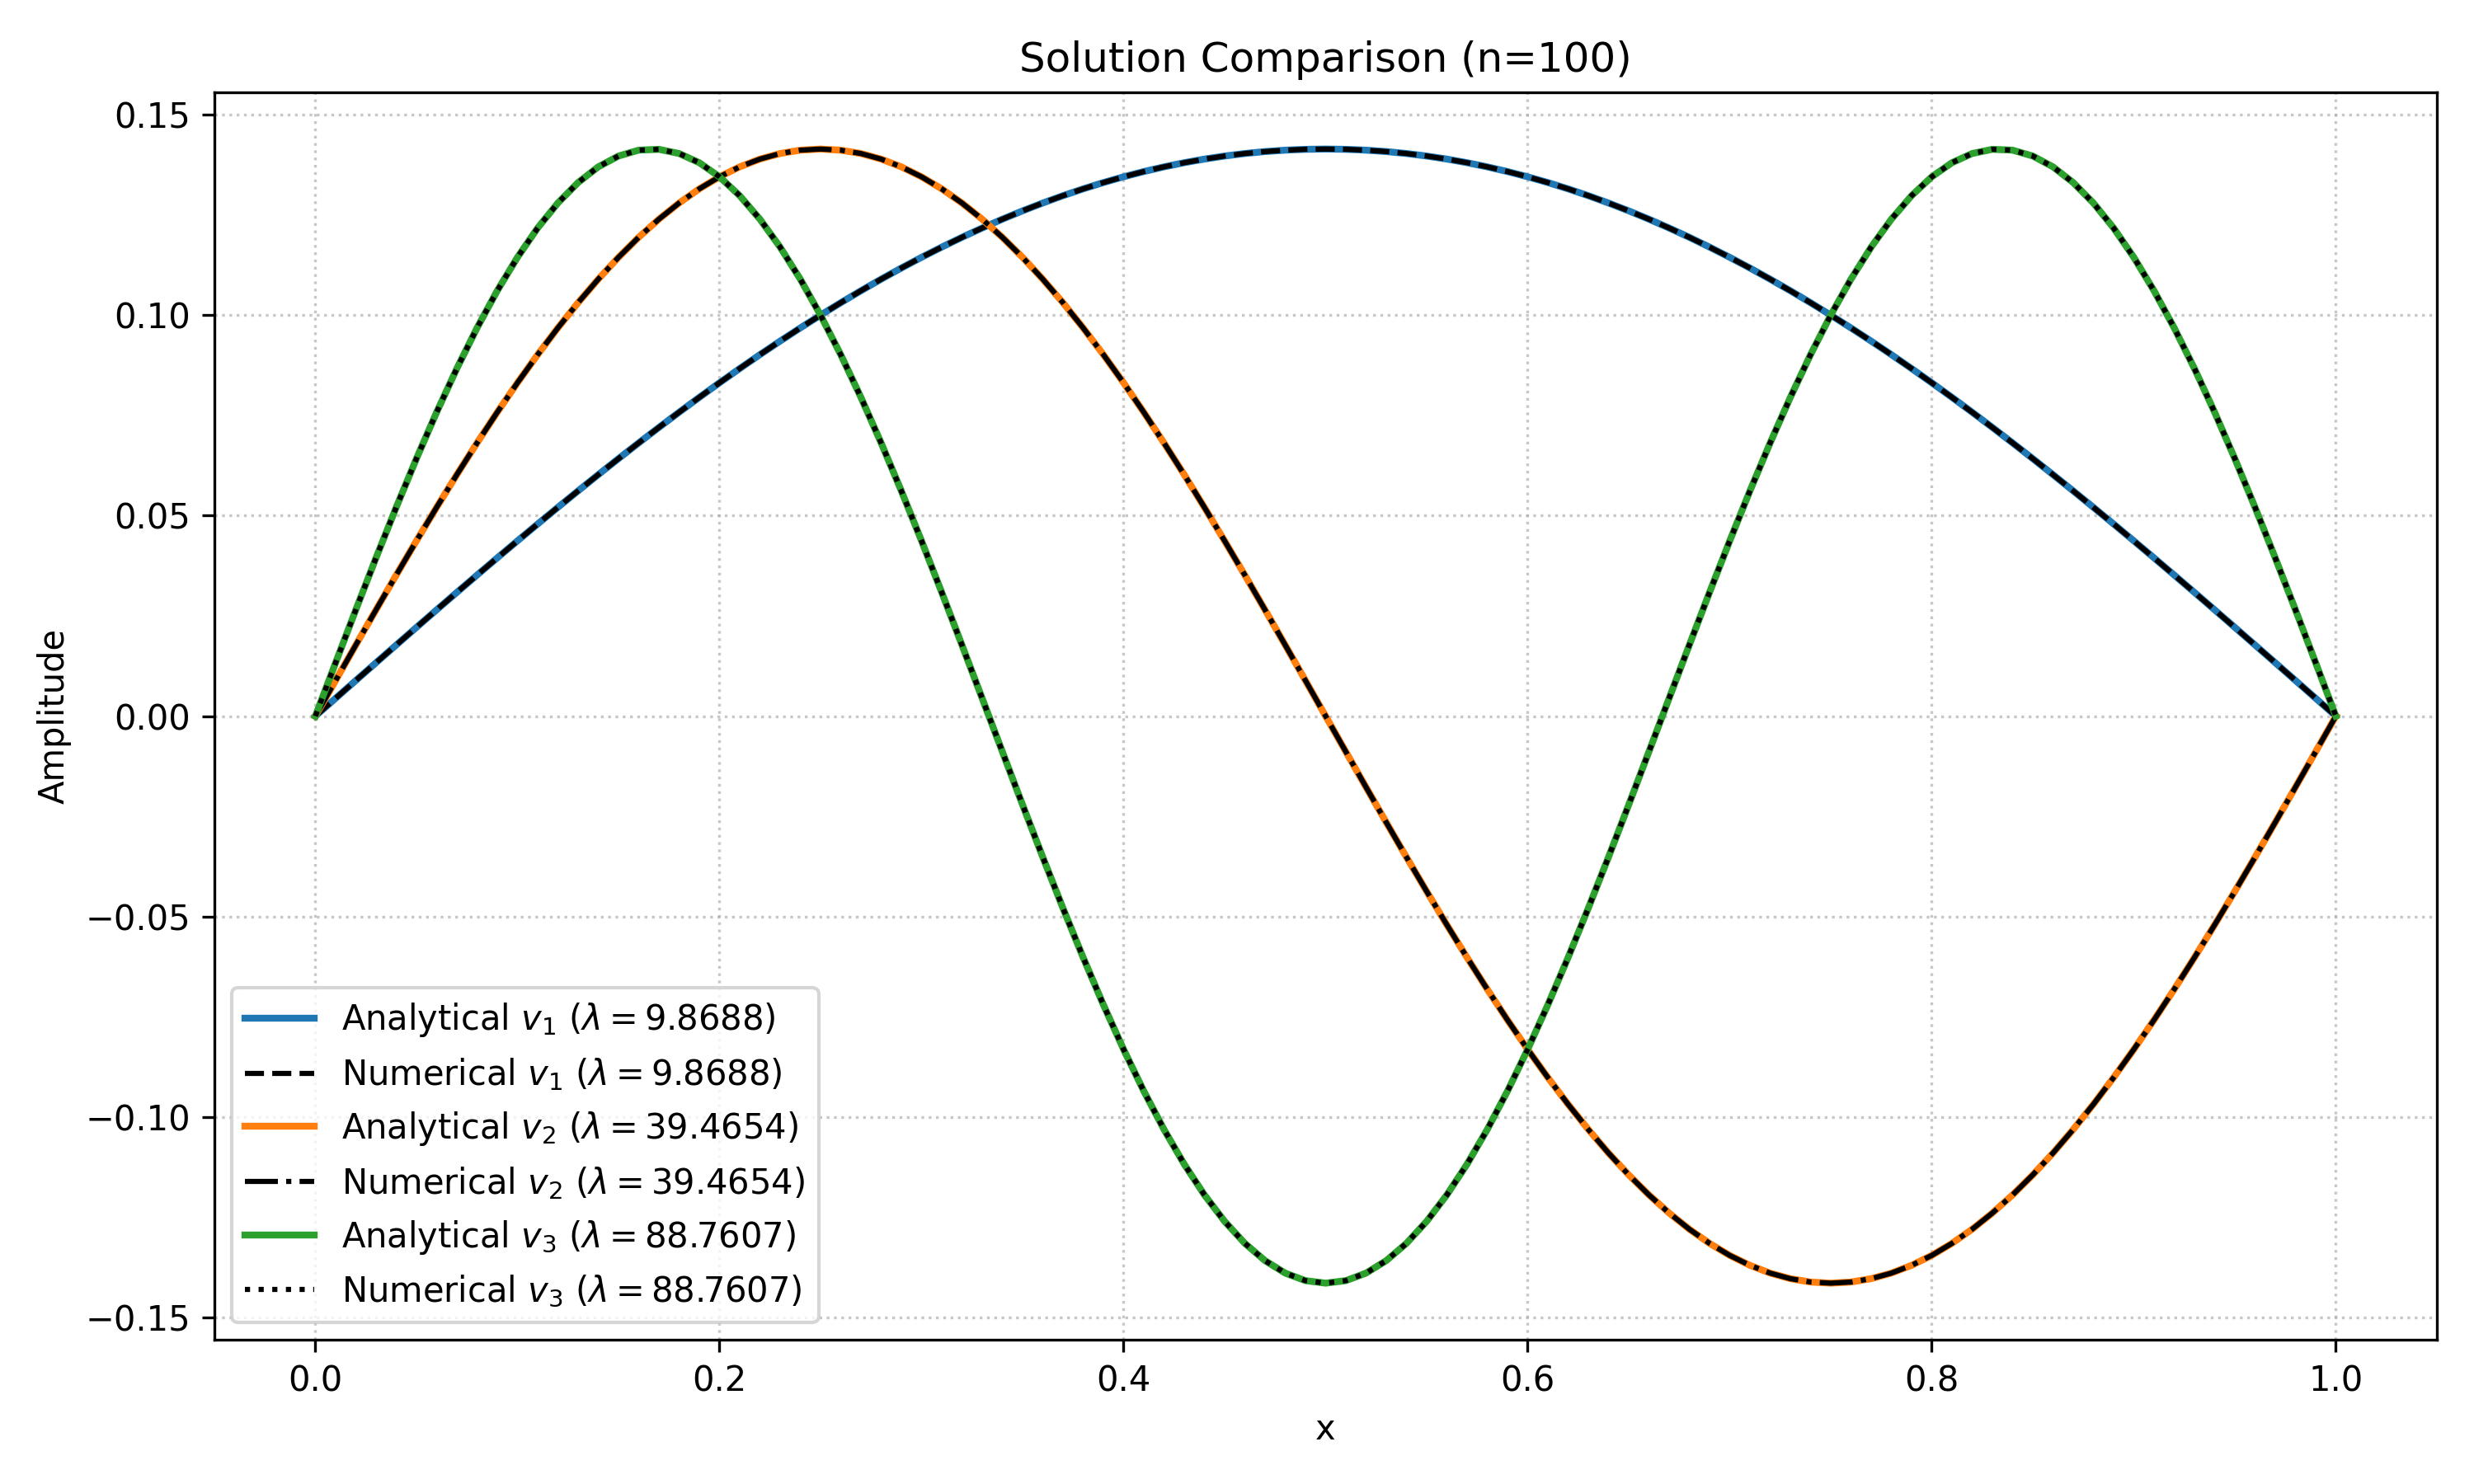
\includegraphics[width=1\textwidth]{task6_100.png}
%         \caption{Relative error comparison, problem 8b}
%     \end{subfigure}
    
%     \caption{Comparison of absolute and relative errors between exact and numerical solutions}
% \end{figure}

\bibliography{references}
\end{document}